\documentclass{ximera}
\input{../preamble.tex}

\author{D. Davis \and R. Speckert \and N. Shay \and A. Davis}
\title{Measurement, Data Collection and Representation} \license{CC BY-NC-SA 4.0}
\begin{document}

\begin{abstract}
\end{abstract}
\maketitle

\begin{onlineOnly}
\section*{Measurement, Data Collection and Representation}
\end{onlineOnly}
\subsection*{Background}
Units of measurement are used to represent physical quantities like length, area, volume, mass, temperature, current, voltage, intensity, etc.  There are different measurement units used to represent the magnitude of the physical quantities. The International System of Units (SI Units) are the most widely used across the world. Measurement units compare how large or small a physical quantity is as compared to the basic standard quantity.  

$$\begin{array}{|c|c|c|} 
 \hline \text{Entity}&\text{Base Unit Name}&\text{Abbreviation}\\ \hline \text{Mass}&\text{kilogram}&\text{kg}\\  \text{Length}&\text{meter}&\text{m}\\
 \text{Time} &\text{second}&\text{s}\\
  \hline 
 \end{array}$$

\subsection*{Units}
When collecting and recording data, be sure to always include the correct units.  Also, the units must make sense to the magnitude of the data.  For example, if you were to measure the width of the room in which you are seated, the most logical SI units would be meters and the most logical measuring device would be a meter stick or tape measure.  
Why not record the width of the room in millimeters?  
Recording measurements in units that are logical helps with visualization of the actual size.  
Also, know when the unit is linear, squared, or cubed.   Check these images (not to scale):

\begin{center}
\tdplotsetmaincoords{70}{130}
	\begin{tikzpicture}[scale=0.6]
 \filldraw[white, opacity=1](0,0,2)--(0,4,2)--(0,4,-2)--(0,0,-2)--cycle;
   \filldraw[white, opacity=1] (4,0,2)--(0,0,2)--(0,0,-2)--(4,0,-2)--cycle;
   \filldraw[white, opacity=1] (0,4,2)--(0,4,-2)--(4,4,-2)--(4,4,2)--cycle;
   \filldraw[white, opacity=1] (4,4,2)--(4,4,-2)--(4,0,-2)--(4,0,2)--cycle;
   \filldraw[white, opacity=1] (0,4,2)--(4,4,2)--(4,0,2)--(0,0,2)--cycle;
\draw[line width=1pt](0,0,2)--(4,0,2) ;
\node[] at (1.2, -1.5, 0)   {Length: $1$ meter};
     \end{tikzpicture}\quad\quad
         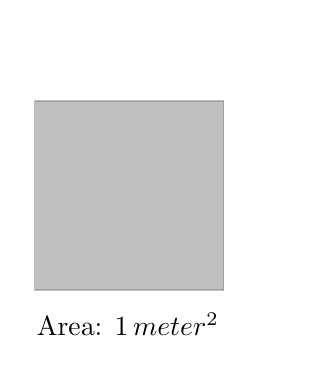
\begin{tikzpicture}[scale=0.6]
\filldraw[white, opacity=1](0,0,2)--(0,4,2)--(0,4,-2)--(0,0,-2)--cycle;
   \filldraw[white, opacity=1] (4,0,2)--(0,0,2)--(0,0,-2)--(4,0,-2)--cycle;
   \filldraw[white, opacity=1] (0,4,2)--(0,4,-2)--(4,4,-2)--(4,4,2)--cycle;
   \filldraw[white, opacity=1] (4,4,2)--(4,4,-2)--(4,0,-2)--(4,0,2)--cycle;
   \filldraw[white, opacity=1] (0,4,2)--(4,4,2)--(4,0,2)--(0,0,2)--cycle;         
\filldraw[gray, opacity=0.5] (0,0,2)--(0,4,2)--(4,4,2)--(4,0,2)--cycle;
\node[] at (1.2, -1.5, 0)   {Area: $1\, \text{meter}^2$};
	\end{tikzpicture}\quad\quad
	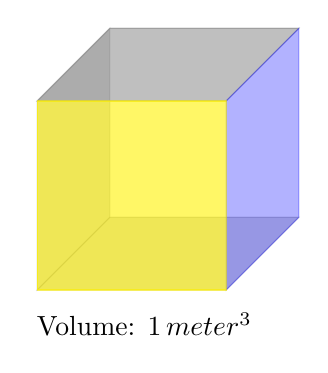
\begin{tikzpicture}[scale=0.6]
   \filldraw[gray, opacity=0.3](0,0,2)--(0,4,2)--(0,4,-2)--(0,0,-2)--cycle;
   \filldraw[gray, opacity=0.3] (4,0,2)--(0,0,2)--(0,0,-2)--(4,0,-2)--cycle;
   \filldraw[gray, opacity=0.5] (0,4,2)--(0,4,-2)--(4,4,-2)--(4,4,2)--cycle;
   \filldraw[blue, opacity=0.3] (4,4,2)--(4,4,-2)--(4,0,-2)--(4,0,2)--cycle;
   \filldraw[yellow, opacity=0.6] (0,4,2)--(4,4,2)--(4,0,2)--(0,0,2)--cycle;
   \node[] at (1.5, -1.5, 0)   {Volume: $1\, \text{meter}^3$};
\end{tikzpicture}
%    \end{center}     
 \end{center}

\begin{question}\label{q:lengthAreaVolume}
    For each example, select an appropriate type of measurement.

    John lives in an $1,800$ sq. ft. house: \wordChoice{\choice{Length}, \choice[correct]{Area},\choice{Volume}}

    Sarah purchases $5$ gallons of paint: \wordChoice{\choice{Length}, \choice{Area},\choice[correct]{Volume}}
\end{question}

\begin{warning}
\begin{itemize}
    \item Units are as important to a measured value as the number. Always include units when recording a measurement. 
\item Make sure the units make sense. For example, don’t give the length of a typical pencil in meters -- instead give the dimension in centimeters or millimeters.
\end{itemize}
\end{warning}

 \subsection*{Units Conversion}

 \begin{example}\label{ex:unitConversion}
     Convert $575$cm to meters. 
     \begin{explanation}
     To do this, multiply $575$cm by a “strategic one”.  
$$575\text{cm}\times \frac{1\text{m}}{100\text{cm}}=\frac{575\cancel{\text{cm}}}{100}\frac{\text{m}}{\cancel{\text{cm}}}=\answer{5.75}\text{m}$$
     \end{explanation}
 \end{example}

 \subsection*{Measurement Process}
 Technicians measure stuff. Therefore, it is important to report a measurement in a meaningful and reliable format.
To do this, the technician must:
\begin{itemize}
\item Select the correct instrument and be knowledgeable of how it works and how to care for it.
\item Calibrate the instrument (transfer standards are traceable to \href{https://www.nist.gov/}{NIST} or other sources).
\item Report  measurement accurately, to a meaningful level of precision, and with proper units.
\end{itemize}

When measuring the thickness of a metal layer resulting from a chemical vapor deposition (CVD), a technician would use a scanning electron microscope \href{https://www.nist.gov/news-events/news/2023/05/leveling-sem-measurements-chip-manufacturing}{(SEM)}.  A SEM is a high precision, delicate instrument that requires training on how to use, care for, and calibrate the device. Many other measuring instruments are used in manufacturing including micrometers, calipers, hardness and surface testers, gauges, and more. 

The accuracy of a measuring instrument is the ability to yield the true or correct value and the precision is the ability to repeat values with small variation. For measuring instruments to be accurate and precise, they must be used correctly, handled and cared for properly, and calibrated. 

Calibration of measuring instruments is crucial to the measurement process. The calibration requirements vary by instrument and applications. Sometimes calibration might be as simple as checking or zeroing the instrument while some instruments used is critical measurement processes may require periodic calibration using standards or transfer standards from the National Institute for Science and Technology (NIST).
    
The degree of precision in reporting a measurement is limited by the least precise measuring instrument used in the process. 
\begin{question}\label{q:lengthOfRoom}
When measuring the width of the room you are in, suppose you used the balsa wood meter stick given to you at the local bank for opening a new account.  When you got near the wall, you pull out the engineer’s scale calibrated to millimeters and report the width of the room to the nearest millimeter.  Is that level of precision valid?  Discuss why or why not?   So how strong is a chain?  A chain is as strong as the weakest link just like a measurement can be no more precise than the least precise measuring instruments used in the process. 
\end{question}

\begin{question}\label{q:equalLength}
When recording a measurement, we write the numeric value to the level of decimal points used in the measurement and include units. Are the following measurements equal?  Explain your answer.   
$$20\text{cm}\quad 20.0\text{cm}\quad 20.00\text{cm}\quad 20.000\text{cm} $$

\begin{multipleChoice} 
\choice{Yes, $20=20.0=20.00=20.000$.} 
\choice{No, (insert silly reason here)} 
\choice[correct]{No, (insert a good reason here)}
\end{multipleChoice} 
\end{question}

\subsection*{Visualizing Manufacturing Data}

Need a better title.  This is where we would talk about the shape of measurement data.

\begin{exploration}\label{exp:histogram1}
Consider a sample of 100 silicon wafers whose thickness of a metal layer resulting from a chemical vapor deposition (CVD) in a semiconductor plant. The data represent the layer thickness on semiconductor wafers measured in angstroms (one ten billionth of a meter).

% \begin{pdfOnly}
% Access GeoGebra interactives through the online version of this text at 

% \href{https://ximera.osu.edu/qcstats}{https://ximera.osu.edu/qcstats}.
% \end{pdfOnly}
CLICK on the SLIDER to change the number of buckets (bars).

\begin{onlineOnly}
\begin{center} 
\geogebra{dhvgryen}{800}{600} 
\end{center}
\end{onlineOnly}

We can see by the histogram output that the data has the triangular shape and symmetry associated with the bell shape. We can say that this sample data is normally distributed.

I'm including this wafer pic just for fun:

\begin{image}
         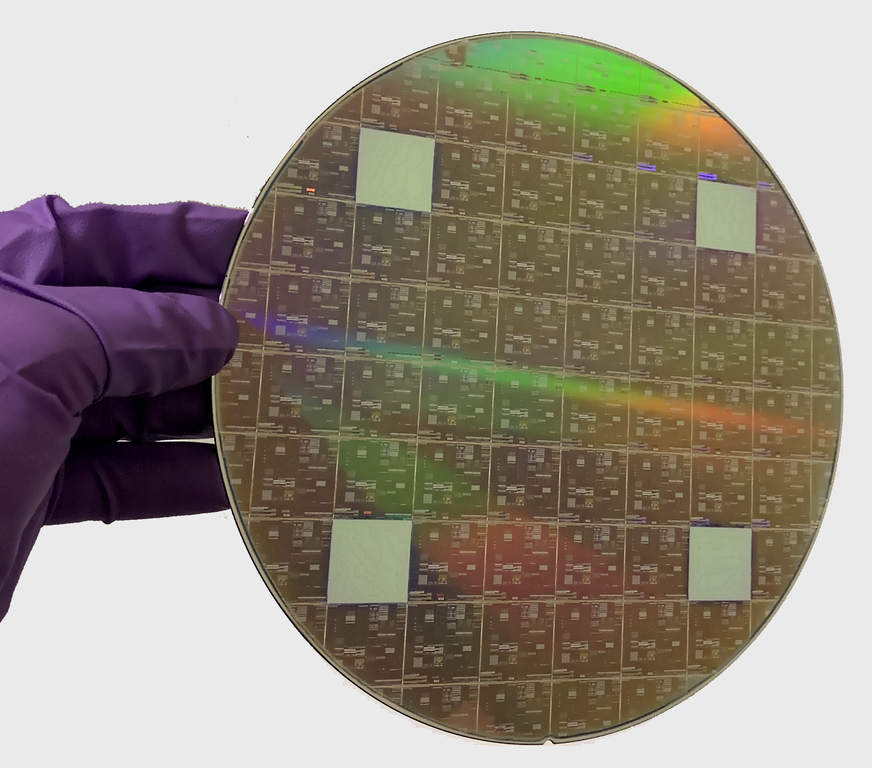
\includegraphics[height=1.5in]{200mmWafer.png}
\end{image}
\end{exploration}

\subsection*{Specification Limits}
Manufactured parts typically have to fit with many other parts, so their measurements matter. Due to natural variation inherent in all manufacturing processes we cannot require a part to have a specific exact measurement.  Instead, we require that the measurement falls within a certain acceptable range based on practical restrictions on how big or small a part can be and still fit with the other parts.  Such restrictions are called \emph{specification limits} or \emph{specs}.  The diagram below breaks the specification limits for the length of a screw into two types.  The \emph{lower specification limit} (LSL) is the shortest length a screw can be to hold the two planks of wood together; the \emph{upper specification limit} (USL) is the longest length a screw can be without sticking out on the other side and potentially causing injury.

\begin{center}
        \begin{tikzpicture}
\node[inner sep=0pt, anchor=base] (p1) at (0,0)
  {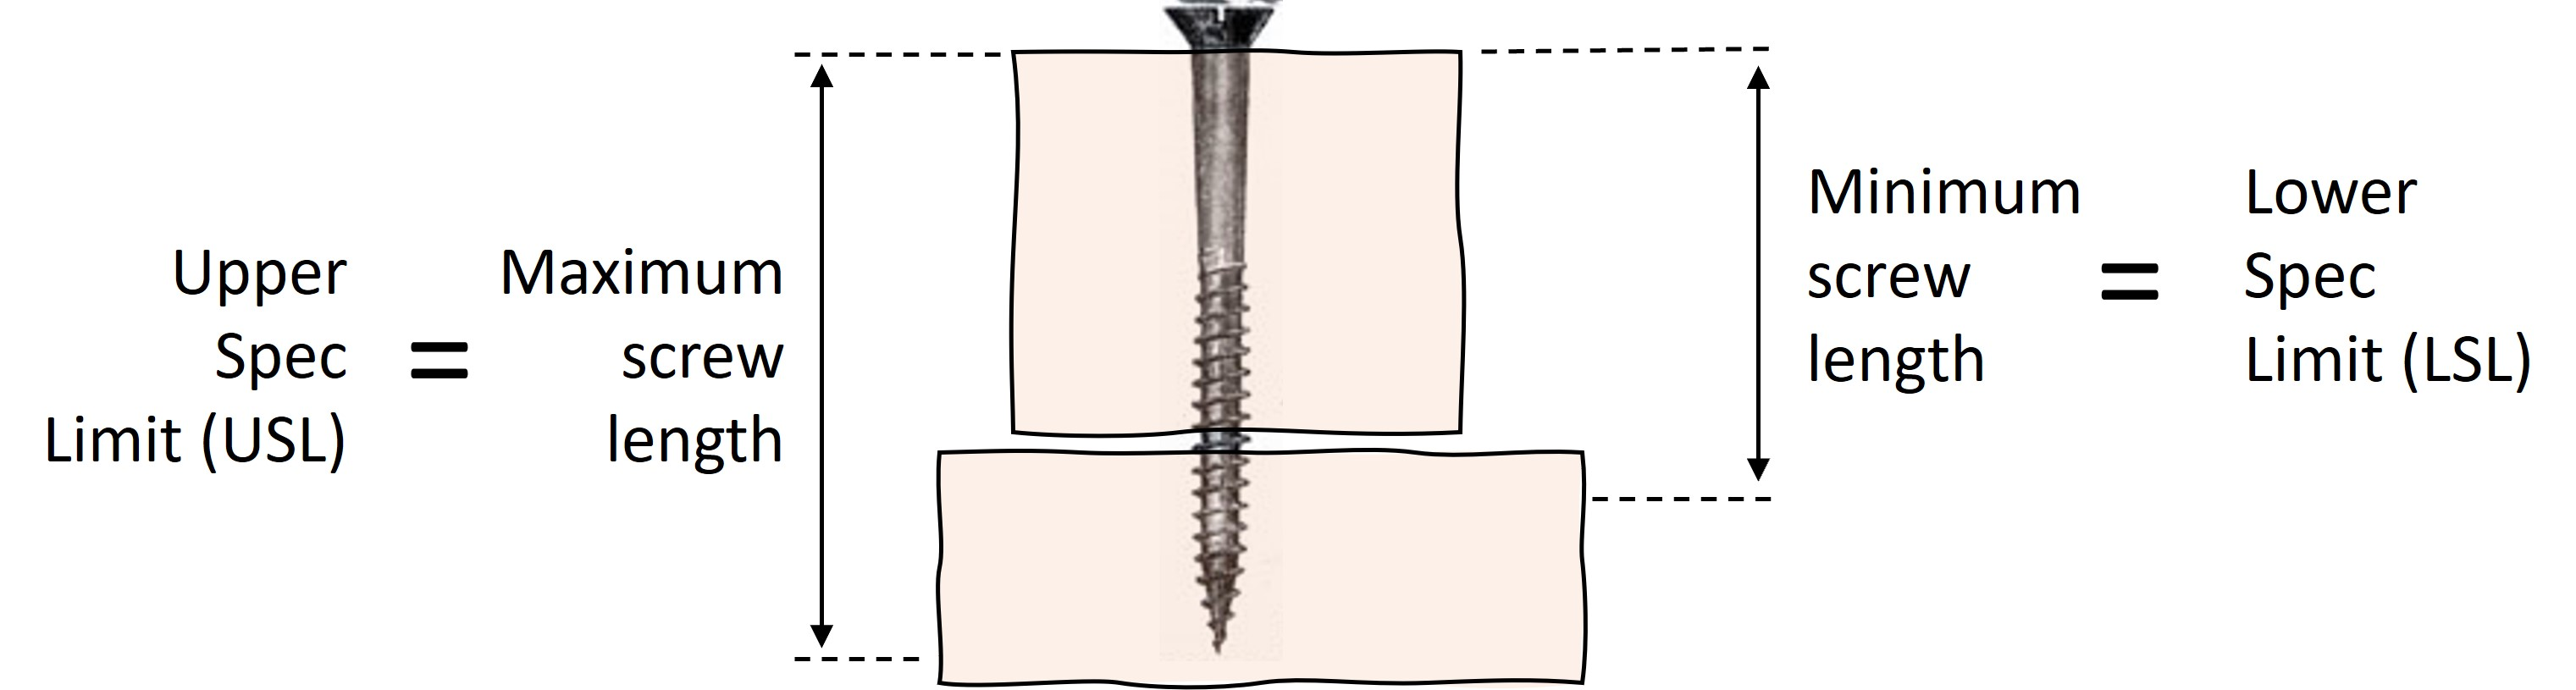
\includegraphics[height=40mm]{screw1.jpg}};
           \end{tikzpicture}
      \end{center}

If a part's measurement falls outside of the specification limits, the part is considered to be \emph{defective} or \emph{scrap}.  For example, we may order a batch of $50$ mm screws with specifications of $50$mm $\pm 6$mm.   Given these specs, a $52$mm screw is okay, but a $43$mm screw is scrap.

\subsection*{Six-sigma quality standard}
Let's return to the large batch of screws example from the previous section.  Recall that we set the specs for screw length to be $50$mm $\pm 6$mm.  

Both fall within specs, but Machine 2 is much better than Machine 1.

\begin{onlineOnly}
\begin{center} 
\geogebra{gtfzbdzs}{900}{600} 
\end{center}
\end{onlineOnly}

\begin{example}\label{ex:defParts1}
    Suppose that the output of Machine 1 can be described using normal distribution with mean $\mu=50$ and standard deviation $\sigma=2$.  If a batch of $1,000,000$ is ordered.  How many defective screws do you expect?
    \begin{explanation}
        Observe that $50-3\sigma=44$ and $50+3\sigma=56$.  By the Empirical Rule, $99.7\%$ of the data lies between $44$ and $56$.  The end-points of this interval just happen to coincide with the spec limits.  Therefore, $99.7\%=0.997$ of output falls within the spec limits.  This may seem like a good thing, but if we fill an order of $1,000,000$ using Machine 1, then the number of defective screws will be approximately
        $$(1-0.997)\times 1,000,000=0.003\times 1,000,000=3,000$$
        
    \end{explanation}
\end{example}


\begin{onlineOnly}
\begin{center} 
\desmos{f95viwzyer}{800}{600} 
\end{center}
\end{onlineOnly}
 





\section*{Practice Problems}

\section*{References}
Wafer photo credit: \textit{Processed 200 mm Si Wafer} by Goldenvu CC BY-SA 4.0.

\end{document} 